% Chapter5

\chapter{Wirtschaftliche Machbarkeit} \label{chapter:Wirtschaftliche Machbarkeit}

\section{Aufwandsabsch�tzung}

\begin{figure}[h]
	\centering
		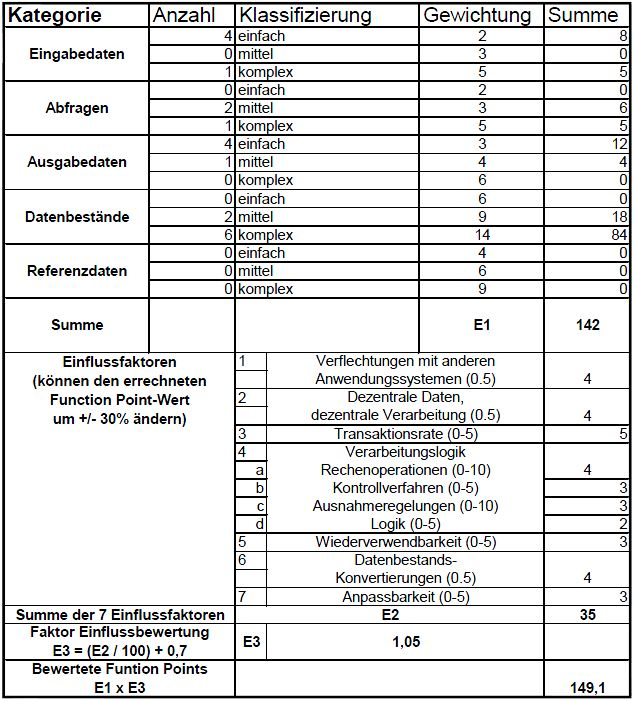
\includegraphics{graphics/chapter5/FunctionPointsAnalysis.JPG}
	\label{fig:FunctionPointsAnalysis}
\end{figure}


\section{Risikoanalyse}
\label{section:Risikoanalyse}

\subsection{Personenausfall}
\label{subsection:Personenausfall}

Eintrittswahrscheinlichkeit:  gering \\
Auswirkungen:  								gering \\

In dem unerwarteten Fall, dass ein Teammitglied l�ngerfristig ausf�llt, muss es m�glich sein die Arbeitsaufgaben dementsprechend neu aufteilen zu k�nnen.
Folgende F�lle k�nnten auftreten:
\begin{itemize}
	\item Streit im Team
	\item Ausfall durch Krankheit oder Tod eines Teammitglieds
	\item Austritt eines Teammitglieds aus dem Projekt
	\item Der Auftraggeber k�nnte aufgrud von Unklarheiten den Projektabbruch initiieren 
	\item Es kann passieren, dass von Seite des Auftragsgebers pl�tzlich kein Interesse an der Umsetzung des Produktes mehr gegeben ist, und es dadurch zu extremem Zeitverzug kommt, was bis zum Abbruch f�hren kann
\end{itemize}

Folgende pr�ventive Ma�nahmen werden eingef�hrt:
\begin{itemize}
	\item Regeln f�r den Umgang innerhalb des Projekts
	\item Ausreichendes Interesse jedes Mitglieds und keine leistungstechnische Probleme 
	\item Gutes Verh�ltnis mit den Auftraggebern
\end{itemize}

\subsection{Zetiliche Risiken}
\label{subsection:Zeitliche Risiken}

Eintrittswahrscheinlichkeit:  gering \\
Auswirkungen:  								mittel \\

Die Aufwands- und Zeitsch�tzung basiert auf dem derzeitigen Lastenheft des Auftraggebers und stellt eine zeitgerechte Fertigstellung sicher. Sollten sich jedoch die Anforderungen des Kunden w�hrend des Projekts �ndern, so wird sich das mit gro�er Wahrscheinlichkeit verz�gernd auf den Fertigstellungstermin auswirken. Die mit dem Kunden vereinbarte Funktionsanalyse und die Meilensteine mit gemeinsam festgelegten Qualit�tskriterien sollten jedoch diesem Risiko entgegenwirken.

\subsection{Technische Risiken}
\label{subsection:Technische Risiken}
\textbf{Datenverlust}\\
Eintrittswahrscheinlichkeit:  gering \\
Auswirkungen:  								mittel \\

Aufgrund der nicht auszuschlie�enden Gefahr des Datenverlusts, muss daf�r gesorgt werden die Sicherheit der Daten, sowie auch die Verf�gbarkeit dieser zu garantieren. Dieses Problem wird mithilfe eines \gls{git} gel��t, durch diesen Server ist es m�glich die Versionen der Software immer zug�nglich zu machen und zus�tzlich die Daten auf den Computern der Projektmitgliedern zu speichern.